\chapter{Estado del Arte}\label{chapter:state-of-the-art}

El objetivo principal del Sistema de Nombres de Dominio es el acceso a recursos en la red a través de un espacio de nombres. Anterior a este, en los años 1970, la red era una comunidad pequeña con unos pocos cientos de computadores. El mapeo del nombre de cada \textit{host} a su dirección era mantenido por el Centro de Información de Red (NIC, por sus siglas en inglés) en un archivo nombrado \verb+HOSTS.TXT+ [\cite{rfc_1034}].

Al aumentar la red aparecen organizaciones y redes administradas de forma local cuyos administradores debían esperar por los cambios que solicitaban aplicar al \verb|HOSTS.TXT| vía correo, para posteriormente descargar el archivo actualizado mediante FTP. Como consecuencia de estas solicitudes aisladas, es posible que se traten de introducir nombres que colisionen. 

% En sistemas de tipo Linux puede encontrarse en la ruta \verb+/etc/hosts+, mientras que en Windows esta ubicado en \verb+C:\Windows\System32\Drivers\etc\hosts+ pues este aún se consulta antes de resolver un dominio con un servidor de nombres.

El hecho de clonar el archivo por todos los \textit{hosts}, trae como consecuencia un alto consumo de ancho de banda y poca escalabilidad ante el aumento del número de dispositivos de cómputo. Cada nuevo punto en la red significa una nueva línea en el archivo y otro posible cliente a quien servirlo. La carga generada en el servidor FTP de NIC es considerable y aumenta de formar cuadrática respecto al número de clientes [\cite{rfc_1034}].

Se hace necesario tener una alternativa a dicho mecanismo. DNS como base de datos distribuida, jerárquica y altamente disponible soluciona dicho problema, además de aportar nuevas funcionalidades.

\section{DNS}

DNS tiene una estructura arbórea, donde cada nodo tiene un padre y una etiqueta de 1 a 63 caracteres de longitud, excepto el nodo raíz que es su propio padre y contiene la cadena vacía [\cite{Vixie_2007}]. Un nombre de dominio puede verse como un nodo en este contexto, mientras que, un nombre de dominio completamente calificado (FQDN, por sus siglas en inglés) es una representación de nodos, separados por un punto (\verb+.+). Por ejemplo, \verb+www.example.com+ es el FQDN para el dominio \verb+www+, cuyo padre es \verb+example+, abuelo \verb+com+ (TLD, del inglés \textit{Top Level Domain}) y bisabuelo el nodo raíz.

En la arquitectura actual encontramos lo dominios de más alto nivel (TLD) un nivel por debajo del nodo raíz. Estos son directamente gestionados por la IANA (\textit{Internet Assigned Numbers Authority}) y la lista se encuentra en la base de datos de la zona raíz\footnote{\url{https://www.iana.org/domains/root/db}}. La administración de los TLD es delegada a empresas y organizaciones en coordinación con la IANA para su mantenibilidad.

\begin{figure}[!ht]
    \centering
    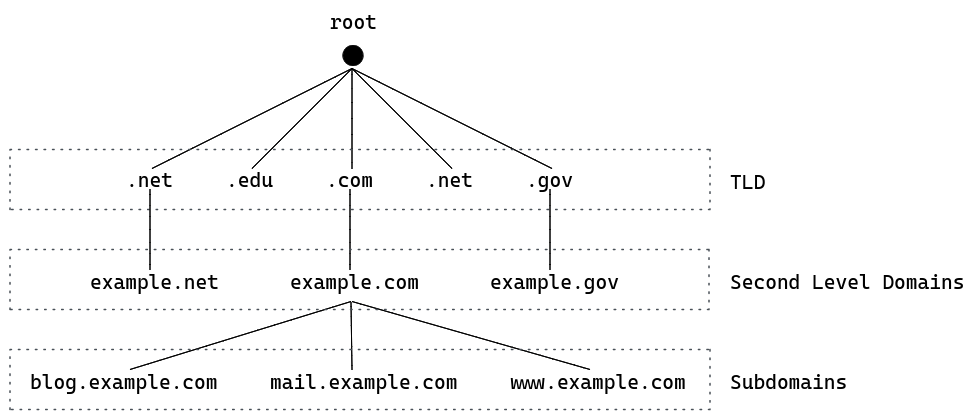
\includegraphics[width=\linewidth]{draws/dns-arch.png}
    \caption{Arquitectura de DNS.}
\end{figure}

Los nodos (dominios) son agrupados en zonas, las cuales pueden considerarse un área dentro del espacio de nombres. Siendo cada zona administrada por una organización o administrador determinado. La zonas son manejadas por servidores de autoridad, que pueden ser \textbf{primarios} (si la información de la zona tiene su origen fuera de DNS) o \textbf{secundarios} (la información tiene como origen un servidor primario, vía una transferencia de zona) [\cite{Vixie_2007}].

Cada nodo puede poseer registros (en inglés \textit{resource records} (RRs)). Estos son los que contienen toda la información DNS en dependencia de su nombre, tipo, clase o datos [\cite{rfc_1035}]. Cada RR tiene un TTL (\textit{time to live}), que indica que tiempo puede estar almacenada la información del registro en un servidor secundario, después de que este llegue a cero es necesario volver a obtener el registro del servidor autoritario primario.

\subsection{Tipos de Consultas DNS}

Como resultado de disponer de una base de datos distribuida, un servidor puede recibir una consulta que solo otro servidor puede responder. Así, una consulta DNS puede ser resuelta por los diferentes servidores que componen la jerarquía de nodos. Comenzando desde el nodo raíz hasta el servidor autoritario que debe contener la información requerida si esta existe.

\begin{figure}[!ht]
    \centering
    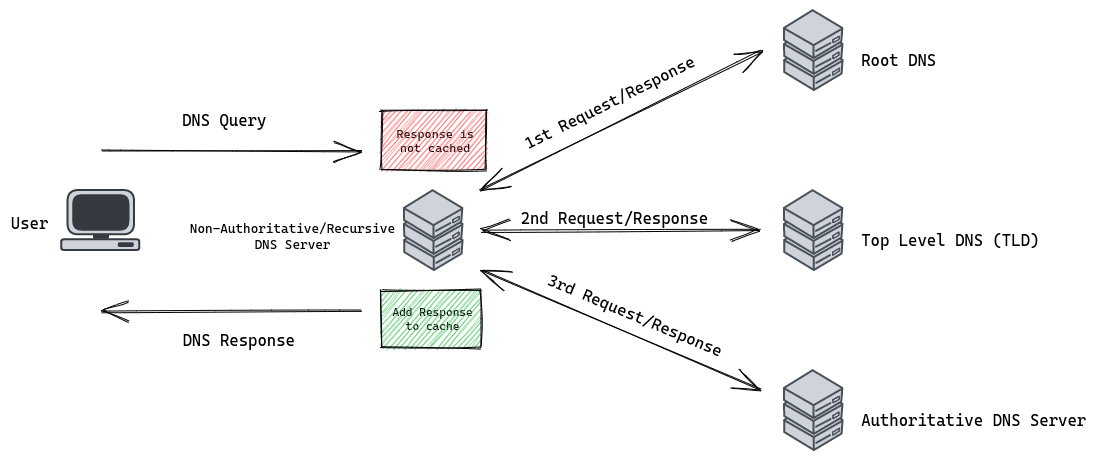
\includegraphics[width=\linewidth]{draws/dns-query.png}
    \caption{Resolución de una consulta DNS.}
\end{figure}

De forma estándar una consulta está compuestas por un dominio objetivo (\verb|QNAME|), un tipo (\verb|QTYPE|) y una clase (\verb|QCLASS|). El servidor DNS usa el \verb|QTYPE| y \verb|QCLASS| para dar respuesta a la consulta con el conjunto de RR relevantes. En adición a los registros retornados, el servidor puede apuntar a otro servidor de nombres que tiene información relevante para la consulta o útil para interpretar la información dada como respuesta.

Existen dos tipos de consultas (no confundir con \verb|QTYPE|), de acuerdo al proceso que realizan los servidores para dar la respuesta. Estas son recursivas e iterativas. Son dos aproximaciones distintas para resolver la obtención de información en una base de datos jerárquica y distribuida. DNS requiere la implementación de la solución iterativa y deja de manera opcional la recursiva [\cite{rfc_1034}].

En una consulta recursiva el cliente DNS provee el nombre de un host y el \textit{DNS Resolver} es el encargado de darle respuesta con un registro relevante o un mensaje de error en el caso que no fuera encontrado. El \textit{resolver} inicia esta consulta comenzando desde el servidor raíz, hasta que encuentre el servidor de nombres autoritario para la consulta, el cual contiene la dirección IP u otra información con la que dar respuesta.

Por otra parte, la consulta iterativa comienza cuando el cliente DNS provee el nombre de un host y el \textit{DNS Resolver} debe darle la mejor respuesta que tenga, dígase apuntarlo al servidor de nombres más probable de contener la respuesta a la consulta. Si el \textit{resolver} tiene el registro relevante para la consulta en su caché, este valor es dado como respuesta, sino el cliente es referido al servidor DNS raíz u otro servidor de nombres autoritario que sea más cercano a la zona deseada. Así, el cliente debe repetir la consulta al servidor al que fue referido.

\subsection{Registros y Extensibilidad}

Los registros DNS han ido evolucionando a lo largo de los años desde el diseño inicial del sistema. Diferentes RFCs (\textit{Request for Comments}) han ido añadiendo nuevos registros y dejando obsoletos otros. Los principales motivos para estos cambios es añadir nuevas funciones a DNS y mejorar la seguridad del sistema. Otro caso son tipos de registros que aún no son obsoletos pero están en desuso o no son usados por ninguna aplicación notable.

Los registros son el punto final de la jerarquía DNS, donde un nodo puede contener un conjunto de estos, que puede ser vacío. Ante una consulta resuelta por el nodo da como respuesta con un subconjunto de los RR que él mantiene.

Un RR esta conformado por diferentes campos. De forma general, tiene un propietario, que es el nombre de dominio dónde es encontrado, un tipo, algunos de los más comunes son \verb|SOA|, \verb|A|, \verb|NS|, \verb|MX|, \verb|CNAME|, y una clase que indica el protocolo al que pertenece y un TTL. Cada registro tiene finalmente un \verb|RDATA| dependiente de la clase y en ocasiones del tipo, por lo que puede contener información variada. Este puede ser un nombre de dominio, una dirección IP o incluso texto de propósito general, como es el caso del tipo \verb|TXT| [\cite{rfc_1464}].

\subsection{Seguridad}

Una vulnerabilidad de un sistema o una red es cualquier debilidad mediante la cual pueda comprometerse la información o el comportamiento del mismo. Múltiples amenazas pueden hacer uso de debilidades en un servidor DNS que no este configurado apropiadamente y realizar acciones malintencionadas.

DNS en su diseño inicial no esta orientado a la seguridad. Fue creado cuando el tráfico en internet era mucho menor a lo que es ahora y la seguridad no era una de las consideraciones principales. Consecuencia de ello, cuando un \textit{resolver} le envía una petición a un servidor autoritario de zona, no tiene como verificar la autenticidad de la respuesta que recibe. Solo es posible verificar que la dirección IP coincida, pero este no es un mecanismo lo suficientemente fuerte para garantizar la autenticidad, pues la dirección IP puede ser falsificada.

Como resultado de este diseño DNS, es vulnerable a muchos ataques. \textit{Cache poisoning} es una consecuencia directa de la ausencia de un mecanismo para verificar la autenticidad de una respuesta. Un \textit{resolver} puede almacenar en caché una respuesta que fue vulnerada, a partir de este punto responderá a la consulta posteriores con información comprometida, poniendo en peligro a los clientes. Otro riesgo es \textit{DNS Tunneling}, este se desarrolla cuando un atacante es capaz de ejecutar un malware que intercepte la comunicación entre el cliente y el \textit{resolver}. Dado que estas peticiones están autorizadas a pasar el cortafuegos, el atacante también puede pasar por este sin ser bloqueado [\cite{dns-tunneling}]. A la par existen amenazas que afectan este tipo de sistemas de forma general, principalmente ataques de denegación de servicios, ya sean DoS, DDoS (distribuidos) o DRDoS (reflexión distribuida) [\cite{dns-attacks}]. Un ataque de subdominios aleatorios también es un riesgo, consiste en realizar peticiones al servidor de dominios que no existen pero que pertenecen a la zona, gastando así el ancho de banda y los recursos de cómputo del servidor. Similar a este un ataque de NXDOMAIN tiene como objetivo vulnerar la caché de un \textit{resolver} o servidor autoritario, realizando muchas consultas de dominios que no existen, la respuesta a estas es un registro NXDOMAIN que queda almacenado en caché, así puede llenarse la caché, eliminando información relevante, lo cual causa una demora para resolver las consultas de los clientes reales [\cite{dns-attacks-ident-prot}].

Lógicamente, motivo de la importancia de DNS para las empresas y organizaciones con el auge del internet, fue necesario implementar mecanismos de seguridad que hicieran de DNS un sistema más seguro. En marzo de 2005 es publicado el RFC 4033 que propone un mecanismo, DNSSEC (\textit{Domain Name System Security Extensions}), para autenticar el origen de los datos y la integridad de estos ante una consulta. DNSSEC mejora la autenticación en DNS haciendo uso de firmas digitales basadas en criptografía de llave pública. Cada zona tiene un par de llaves pública y privada. El propietario de la zona hace uso de la llave privada para firmar la información DNS que envía. Mientras que la llave pública es usada por el \textit{resolver} para validar la información recibida [\cite{new-approach-dnssec}].

Aún existe un punto débil, y es como un \textit{resolver} puede verificar que la llave pública que esta recibiendo desde un servidor autoritario es auténtica. Para garantizar su autenticidad es usado el par de llaves del servidor padre, así se hace necesario que el padre y cada uno de los ancestros, hasta la raíz, tengan implementado DNSSEC. Afortunadamente desde el año 2010 el servidor raíz hace uso de DNSSEC, pero no todas las zonas en internet lo han adoptado aún [\cite{dnssec-icann}].

Otras vulnerabilidades de DNS son mostradas en la sección siguiente y específicamente como BIND las mitiga.  

\section{BIND 9}

BIND 9 (Berkeley Internet Name Domain versión 9) en un software de código abierto, mantenido oficialmente por el Internet Systems Consortium (ISC). Actualmente cuenta con tres ramas principales: Estable, Soporte-Extendido y Desarrollo. Esta implementado en C y su código disponible en GitLab\footnote{https://gitlab.isc.org/isc-projects/bind9}. Este es de los más consolidados en el mercado actual de soluciones DNS [\cite{dns-survey}; \cite{bind-usage}], con su surgimiento a inicios de la década de 1980 en la Universidad de California en Berkeley.

Posee un amplio abanico de características empleadas en el sistema DNS actual y es muy utilizado al ser primero en su tipo. Este ofrece tanto un servidor DNS autoritario como un DNS \textit{resolver}, así como un grupo de herramientas adicionales para la gestión del servicio DNS. Ambos servidores siguen prácticas de seguridad y ofrecen funcionalidades que garantizan su correcto funcionamiento al realizar el despliegue en cualquier red.

\subsection{DNS Autoritario}

El DNS autoritario tiene soporte para DNSSEC, lo cual permite ponerlo en producción con un alto esquema de seguridad y que nodos hijos puedan implementar DNSSEC por igual. Este servidor puede tener diferentes roles de acuerdo a la arquitectura usada en el despliegue. Estos roles son Primario, Secundario y Secundario Stealth. Esta arquitectura es escalable, es posible tener un servidor primario (maestro), como fuente de información para la zona, y uno o más servidores secundarios (esclavos). De esta forma los archivos de zona son actualizados en el servidor primario, mientras que los secundarios mantienen copias para responder a consultas.

La transferencia de información entre los servidores de la zona puede ser originada por el servidor primario ante un cambio. Dicho servidor envía un mensaje de tipo \verb+NOTIFY+ a los servidores secundarios, así estos son enterados de que deben realizar una transferencia de zona. Esta transferencia es configurable y puede ser realizada tanto de forma parcial (AXFR), como incremental (IXFR), haciendo uso de TSIG estándar como mecanismo de seguridad.

Las consultas de tipo \verb+ANY+ pueden obtener más información de la que envían, lo que las hace eficaces para efectuar DDoS. El servidor autoritario tiene un mecanismo para protegerse ante esta amenaza, retornando un conjunto predefinido de registros y no todos. BIND 9 usa \textit{rate-limiting} como mecanismo para prevenir ataques de amplificación (un tipo de RDDoS), este puede ser configurado en las opciones o en el ámbito de una vista. Los ataques de amplificación pueden ser evitados con las DNS \textit{Cookies} [\cite{rfc_7873}], estas permiten evitar IPs falsificadas en las consultas y como consecuencia que el servidor no sea involucrado en un ataque de reflexión.

Ante cambios en la configuración de las zonas es posible reiniciar el servidor usando la herramienta de línea de comandos \verb+rndc+ (\textit{remote name daemon control}). \verb+rndc+ permite cargar todas las zonas o especificar cuál, lo cual puede mejorar el tiempo de recarga de la configuración. Además se encarga de remover las zonas eliminadas al recargar la configuración. Esto es la forma más segura de efectuar el proceso, no es necesario reiniciar el servicio y la nueva información de las zonas es enviada a los servidores secundarios si existen.

\verb+dnstap+\footnote{\url{https://github.com/dnstap}} es una solución de código abierto para capturar y \textit{loguear} tráfico DNS. Es soportado por varios servidores DNS de código abierto, entre ellos BIND. Permite capturar el tráfico tanto de consultas como de respuestas del servidor con un impacto menor al \textit{logging} nativo de BIND. La información capturada es almacenada en formato binario, por lo que se ofrece para presentarla de forma legible la herramienta \verb+dnstap-read+. 

\subsection{DNS Resolver}

El DNS \textit{resolver} en BIND también posee funcionalidades que lo hacen muy potente y seguro. DNSSEC viene incorporado y se puede activar de manera sencilla. En caso que exista un problema con el DNSSEC del servidor autoritario puede ser ejecutado el \textit{resolver} con este deshabilitado, haciendo uso de \textit{Negative Trust Anchors} [\cite{rfc_7646}].

Uno de los aspectos más vulnerables y eficaces de los resolvers es la caché. El \textit{resolver} the BIND permite de forma flexible modificar los registros almacenados en caché. Esto puede resultar útil si los datos en caché son incorrectos o están desactualizados. Además, dispone de \textit{cache prefetch}, este mecanismo obtiene desde el servidor autoritario registros que son de frecuente acceso pero que tienen un TTL bajo, mejorando def forma efectiva los \textit{hits} en caché.

Para prevenir ataques DDoS el \textit{resolver} presenta dos opciones de configuración: \verb+fetches-per-zone+ y \verb+fetches-per-server+. Ambas limitan la cantidad de consultas a los servidores autoritarios que puedan estar bajo ataque y de esta forma mitigar la amenaza por la ruta del \textit{resolver}.

Una característica única en BIND es la posibilidad de configurar diferentes vistas en un mismo servidor. Esto permite mostrar a lo usuarios de una red interna y externa (como internet) diferente información DNS, manteniendo cierta información privada. También BIND, de forma particular, ofrece RPZ [\cite{rpz}] (\textit{Response Policy Zone}), estas son zonas diseñadas con un grupo especifico de reglas. Son especialmente usadas para bloquear el acceso a dominios que son conocidos por abuso o actividades ilegales.

\subsection{Alternativas}

Como fue mencionado en la Motivación, existen alternativas a BIND 9. En la tabla a continuación se muestra alguna de ellas.

\begin{table}[!ht]
    \centering
    \begin{tabular}{|l|c|c|c|c|c|}
    \hline
        Software & Pago & API HTTP & UI & Nube & Código Abierto \\ \hline
        BIND 9 & $\times$ & $\times$ & $\times$ & $\times$ & \checkmark \\ \hline
        PowerDNS & $\times$ & \checkmark & $\times$ & $\times$ & \checkmark \\ \hline
        CoreDNS & $\times$ & $\times$ & $\times$ & $\times$ & \checkmark \\ \hline
        Knot & $\times$ & $\times$ & $\times$ & $\times$ & \checkmark \\ \hline
        Amazon Route 53 & \checkmark & \checkmark & \checkmark & \checkmark & $\times$ \\ \hline
        DNS Made Easy & \checkmark & \checkmark & \checkmark & \checkmark & $\times$ \\ \hline
        Google Cloud DNS & \checkmark & \checkmark & \checkmark & \checkmark & $\times$ \\ \hline
        DNSimple & \checkmark & \checkmark & \checkmark & \checkmark & $\times$ \\ \hline
        NS1 & \checkmark & \checkmark & \checkmark & \checkmark & $\times$ \\ \hline
    \end{tabular}
    \caption{Comparativa de soluciones DNS.}
    \label{dns-comparative}
\end{table}

Tanto los servidores de código cerrado, como los de código abierto son mantenidos por instituciones. Los primeros poseen por lo general interfaces de usuario y son gestionados como SaaS (\textit{Software as a Service}). Permiten escalabilidad y acceso a personas sin conocimientos de administración de sistemas a la configuración del servidor DNS. Los proyectos abiertos son más orientados al perfil de administrador de sistemas, donde un conocimiento detallado de la tecnología es necesario.

En este escenario puede hacerse complejo para las organizaciones mantener una arquitectura DNS sin incurrir en gastos de licencia o de personal calificado. Se hace necesario constantemente la intervención de profesionales para modificar la configuración. Una ventaja de poseer el servidor en infraestructura propia y privada es que es más seguro que tenerlo expuesto a internet.

% https://doc.powerdns.com/authoritative/http-api/index.html
En el caso de PowerDNS\footnote{\url{https://github.com/PowerDNS/pdns}}, existe una API HTTP para manejar las zonas del DNS autoritario. Además acepta diferentes tipos de backends, incluyendo los archivos de configuración de BIND para las zonas. Por tanto una implementación para BIND, tentativamente sería aplicable a PowerDNS y otros productos de código abierto.

CoreDNS\footnote{\url{https://github.com/coredns/coredns}}, en su lugar, es muy flexible y la mayor parte de su funcionalidad es derivada de plugins. Actualmente, las instalación por defecto cuenta con más de 30 plugins, pero existen muchos externos y la posibilidad de escribir nuevos para funcionalidades concretas.

Knot\footnote{\url{https://gitlab.nic.cz/knot/knot-dns}} es un servidor DNS solo autoritario con un alto rendimiento, escrito en C. Soporta las características fundamentales del DNS actual, así como reconfiguración en tiempo de ejecución. El software esta orientado a sistemas operativos de tipo POSIX y su desarrollo va enfocado a las necesidades de la comunidad y usuarios donantes al proyecto.

En el grupo de SaaS se encuentra Amazon Route 53\footnote{\url{https://aws.amazon.com/route53/}} con características esenciales para el internet actual. Dispone de cortafuegos para el \textit{resolver}, control de recuperación ante fallos, flujo de tráfico basado en geoproximidad, latencia, salud y otras consideraciones. Como es de esperar, soporta DNSSEC y hace uso de una interfaz gráfica en la web que permite realizar la gestión DNS sin manejar código o archivos de configuración. También ubicado en su propio ecosistema, muy rico en soluciones, está Google Cloud DNS, con características semejantes a las ofrecidas por el producto de Amazon: IAM (\textit{Identity Access Management}), \textit{logging}, DNSSEC, zonas privadas, integración nativa con Kubernetes, y muchas otras.

Los demás servicios de pago como DNS Made Easy\footnote{\url{https://dnsmadeeasy.com/}}, DNSimple\footnote{\url{https://dnsimple.com/}} y NS1\footnote{\url{https://ns1.com}}, también ofrecen registro de nombres de dominio, API HTTP e interfaz web para su gestión. Los SaaS son especialmente útiles para empresas que posean un mercado estable y quieran dedicar menos tiempo a la gestión DNS. Además de mayor seguridad y margen de expansión haciendo uso de sistemas altamente escalables.

% TODO: Describe DNS Made Easy

% TODO: Describe Google Cloud DNS

% TODO: Describe DNSimple

% \section{API REST}

% \subsection{Métodos Alternativos}

\section{Desarrollo Web}

TODO

Las opciones de tecnologías para el desarrollo web actual son bastante amplias. La mayoría de los lenguajes de alto nivel tienen \textit{frameworks} o bibliotecas que facilitan el desarrollo. En desarrollo \textit{front-end} JS/TS\footnote{\url{https://www.typescriptlang.org/}} es el estándar, para \textit{back-end}, las principales diferencias en desarrollo y producción son introducidas por el lenguajes usado. La mayoría de las soluciones existentes en Python, C\#, Java, JS/TS, Go son de código abierto y vienen cargadas de características para disímiles escenarios de implementación.

\subsection{Golang}

Go es un lenguaje compilado con tipado estático diseñado en Google, para el año 2007, por Robert Griesmen, Rob Pike y Ken Thompson. Fue desarrollado para afrontar los retos ingenieriles a los que se enfrentaban los ingenieros en Google. A día de hoy, desde su publicación en 2009, ha alcanzado una adopción masiva y empresas como Cloudflare, Dropbox, Meta, Microsoft, Netflix, PayPal, Twitter, Salesforce, Uber, entre otras, hacen uso de este lenguaje para servir millones de pedidos en escenarios de alta concurrencia con alta disponibilidad. [\cite{go-docs}]

La biblioteca estándar por si sola ofrece las herramientas necesarias para desarrollar una aplicación web. \textit{Encoding} y \textit{decoding} de JSON, validación de datos, implementación de cliente y servidor HTTP, sistema de plantillas HTML seguro contra inyecciones de código, \textit{drivers} para las bases de datos mas usadas, son algunas de las funcionalidades que vienen con el lenguaje.

Existen web frameworks de código abierto, enfocados en el rendimiento y el rápido prototipado, para ayudar en el desarrollo web. Gin\footnote{\url{https://github.com/gin-gonic/gin}}, Buffalo\footnote{\url{https://github.com/gobuffalo/buffalo}}, Echo\footnote{\url{https://github.com/labstack/echo}}, Flamingo\footnote{\url{https://github.com/i-love-flamingo/flamingo}} son algunos de ellos. También de parte de la comunidad podemos encontrar ORMs (\textit{Object Relational Mapper}) como GORM\footnote{\url{https://github.com/go-gorm/gorm}}, para la autenticación web Goth\footnote{\url{https://github.com/markbates/goth}}, con un número amplio de métodos [\cite{goth}], así como implementaciones de JWT (\textit{JSON Web Token}) en el lenguaje.

El método de concurrencia que usa Go es uno de los aspectos fundamentales al considerar el lenguaje. Las llamadas gorutinas (\textit{goroutines} en inglés) son un mecanismo poderoso de concurrencia, más ligeras que los hilos, con solo 2KB en tamaño. Un hilo puede tener cientos de gorutinas ejecutándose. La comunicación entre estas es a través de canales (\verb+chan+), vía de Go para recibir y enviar información entre las gorutinas.

Con la versión 1.18 de Go se añadió genericidad [\cite{go-generics}] al lenguaje, poderosa característica que permite ampliar la reusabilidad del código y la eficiencia durante el desarrollo. El manejo de memoria en Go, es realizado de forma automática por el recolector de basura. El impacto de este sobre el rendimiento es menor y añade más seguridad y portabilidad al software que el manejo manual de la memoria.

El lenguaje hace uso de paquetes para separar el código lo que ayuda a la separación de conceptos y hace uso de un desarrollo enfocado a bibliotecas. De esta forma diferentes proyectos pueden ser desarrollados sobre otros. La compilación en Go se realiza a un solo binario y es más rápida que en otros lenguajes compilados. Las dependencias se encuentran de forma explícita en el código lo que permite realizar la compilación y unión de estas de forma más rápida. En un escenario donde \verb+A.go+ depende de \verb+B.go+ y este de \verb+C.go+, pero \verb+A.go+ no de \verb+C.go+, el compilador primero compila \verb+C.go+, luego \verb+B.go+, y finalmente \verb+A.go+, adicionalmente para compilar \verb+A.go+ se usa \verb+B.go+, no \verb+C.go+ [\cite{go-deps}]. Esta aproximación disminuye considerablemente el tiempo de compilación en proyectos con muchas dependencias.

Para facilitar el desarrollo podemos encontrar de forma predeterminada en el lenguaje varias utilidades: manejo de dependencias, generación de documentación con ejemplos, formateo del código, automatización de tests y \textit{profiling}, son las principales. También es posible analizar los binarios puestos en producción a través de un servidor HTTP [\cite{go-pros-cons}].

\subsubsection{APIs con Go}

Como fue mencionado, existen diferente bibliotecas y frameworks para el desarrollo de servicios HTTP. Este entorno es bastante maduro pues el principal uso del lenguaje es escribir aplicaciones de \textit{back-end}.

Buffalo es un ecosistema para el desarrollo web, actualmente en su version 1.0.1 cuenta con herramientas para generar el la estructura inicial de un proyecto, un ORM con generación automática de modelos, migraciones y configuración para la base de datos. Viene listo para trabajar con tecnología front-end pero también tiene como opción generar un proyecto con el objetivo de servir una API REST HTTP. Podemos encontrar por defecto \textit{hot code reloading} y soporte para realizar \textit{testing}.
              
Echo se autoproclama de alto rendimiento, extensible y minimalista. Este framework dispone de forma predeterminada de un amplio número de \textit{middlewares} que cubren muchos escenarios comunes en el desarrolla de una API o servidor HTML, además de, TLS (\textit{Transport Layer Security}) de forma automática, control de direcciones IP de clientes e integración con cualquier sistema de plantillas. La documentación contiene un índice de referencias con guías paso a paso para diferentes soluciones que se pueden implementar sobre framework, siendo así un buen punto de consulta.

Flamingo es un framework bastante joven, cuenta con poco más de 300 estrellas en GitHub. Está más bien enfocado al desarrollo de aplicaciones \textit{full-stack} que a la implementacion de APIs. Dispone de un poderoso motor de plantillas, diseño orientado a microservicios y escalabilidad en el rendimiento. Además, posee un arsenal de características para la implementación de plataformas de comercio en línea, adaptables a las necesidades de negocio.

Finalmente Gin, con más de 63800 estrellas en GitHub es uno de los frameworks más usados. Semejante a los anteriores, ofrece alto rendimiento, soporte para \textit{middlewares} y extensión de estas, y manejo de errores. Gin captura errores  de pánico y se recupera de estos, de esta forma el servidor siempre esta disponible. El soporte para validación de JSON viene integrado, así como la renderización de plantillas.

Puede concluirse que Go tiene un ambiente con bastas opciones para el desarrollo web. Los frameworks, aunque algunos más consolidados que otros, comparten varias características comunes: extensibilidad, validación de datos, \textit{middlewares} y el alto rendimiento típico del lenguaje. Estas cualidades junto con las herramientas estándar que ofrece el lenguaje hace del desarrollo un proceso bien definido a la hora de afrontar un nuevo proyecto.

\subsection{Vue.js}

Vue.js\footnote{\url{https://github.com/vuejs/core}} es un framework progresivo de código abierto para crear interfaces de usuario en la web con Javascript. Es creado por Evan You después de trabajar para Google en varios proyectos con AngularJS. Vue tiene características similares a Angular, pero con una sintaxis más concisa y sencilla de usar. De igual forma ha adoptado ideas de otros frameworks y bibliotecas como React. [\cite{vue-docs}]

Ofrece un modelo de programación declarativo y basado en componentes que ayuda a desarrollar interfaces de usuario, tanto simples como complejas, de manera flexible. La comunidad ha desarrollado muchas bibliotecas opcionales que son activamente mantenidas, como son: Vue Router (enrutador para crear aplicaciones \textit{single-page}, SPA, por sus siglas en inglés), Pinia (biblioteca para manejo de estado), Vue Server Renderer (biblioteca para renderizado del lado del servidor), entre otras.

El framework ha ido cambiando de manera progresiva (como proclama su eslogan) y adoptando nuevas características. Con Vue 3 se introduce Compostion API como alternativa al estilo establecido por Options API. Ambos estilos son capaces de cubrir los casos de uso, sin embargo Option API esta desarrollada sobre Composition API. Por tal motivo, esta última ofrece más flexibilidad para crear patrones más específicos a la hora de organizar el código y reusar la lógica.

\hspace{-0.65cm}\begin{minipage}{0.5\textwidth}
    \begin{lstlisting}[basicstyle=\ttfamily\tiny, numbers=none, caption=Options API.]
<script>
export default {
// Properties returned from data() become reactive state
// and will be exposed on `this`.
data() {
    return {
    count: 0
    }
},

// Methods are functions that mutate state and trigger updates.
// They can be bound as event listeners in templates.
methods: {
    increment() {
    this.count++
    }
},

// Lifecycle hooks are called at different stages
// of a component's lifecycle.
// This function will be called when the component is mounted.
mounted() {
    console.log(`The initial count is ${this.count}.`)
}
}
</script>

<template>
<button @click="increment">Count is: {{ count }}</button>
</template>
    \end{lstlisting}
\end{minipage}
\begin{minipage}{0.5\textwidth}
    \begin{lstlisting}[basicstyle=\ttfamily\tiny, numbers=none, caption=Composition API.]
<script setup>
import { ref, onMounted } from 'vue'

// reactive state
const count = ref(0)

// functions that mutate state and trigger updates
function increment() {
    count.value++
}

// lifecycle hooks
onMounted(() => {
    console.log(`The initial count is ${count.value}.`)
})
</script>

<template>
    <button @click="increment">Count is: {{ count }}</button>
</template>
    \end{lstlisting}
\end{minipage}

\subsubsection{Reactividad}

La reactividad es una de las principales características de Vue. Con esta cada componente mantiene una referencia a sus dependencias reactivas. De esta forma es posible para el sistema saber cuando renderizar o cual componente renderizar.

En vainilla Javascript no es posible detectar cuando una variable local es leída o modifica. Vue hace uso de proxies (con objetos reactivos) o \textit{getters} y \textit{setters} (con \textit{refs}) para detectar dichos eventos y realizar el renderizado de la parte de la componente afectada.

\subsubsection{Enrutamiento} 

El enrutamiento en el lado del cliente es uno de los puntos fuertes de Vue. Permite crear SPAs que ofrecen una navegación más fluida al no cargar el HTML completo de la página para cada vista. La biblioteca Vue Router es oficialmente soportada por Vue y ofrece completa funcionalidad para implementar la navegación en el lado del cliente.

Las peticiones al servidor son realizadas de acuerdo a la componente que es cargada, dejando libre a este de tener que generar HTML. Por lo general, el servidor solo debe disponer de una API REST o similar para servir la información a la página web.

\subsection{Docker}

Docker brinda la capacidad de empaquetar y ejecutar una aplicación en un entorno aislado llamado contenedor. Los contenedores son livianos y contienen todo lo necesario para ejecutar la aplicación, por lo que no usan las dependencias instaladas en el \textit{host}. Un contenedor es creado a partir de una imagen, y estas se pueden compartir fácilmente asegurando que todas las personas que la reciben obtengan una versión que funciona de la misma manera. Adicionalmente permite manejar la infraestructura de la misma forma que se manejan las aplicaciones, lo que disminuye el tiempo entre escribir el código y llevarlo a producción. [\cite{docker-docs}]

Docker hace especial uso de las características de Linux para el aislamiento de los contenedores, específicamente \verb|namespaces| para el aislamiento de los recursos del host y \verb|cgroups| para el control y limitación de esos recursos. A diferencia de una máquina virtual (MV) que realiza la virtualización sobre el hardware, un contenedor es un proceso corriendo en el sistema operativo, y como resultado se realiza la virtualización sobre este.

\begin{figure}[!ht]
    \centering
    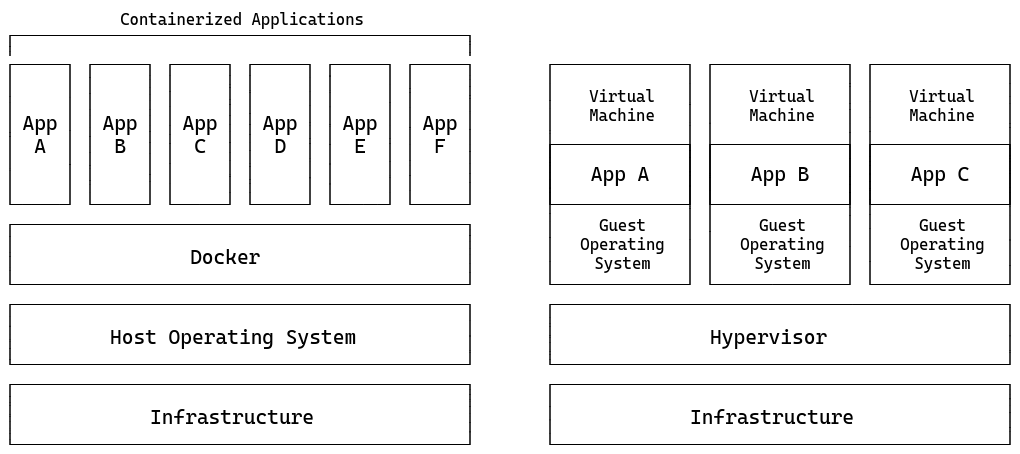
\includegraphics[width=\linewidth]{draws/cont-vs-vm.png}
    \caption{Comparación del funcionamiento de los contenedores y las MV. [\cite{docker-containers}]}
\end{figure}


La adopción de Docker es notable, existen alternativas como Podman, LXD, y Buildah, pero un número considerable de equipos y empresas escogen a Docker para la contenedorización de las aplicaciones [\cite{docker-usage}]. Este es de código abierto y gratis para proyectos de individuos, educación, pequeñas empresas y comunidades de código abierto.

El entorno en que se encuentra Docker es muy rico, dispone de DockerHub\footnote{\url{https://hub.docker.com}}, un sitio para almacenar imágenes, tanto públicas como privadas, lo que ofrece rápido acceso desde cualquier computadora a una imagen que haya sido subida. Estos repositorios son usados por las principales empresas distribuidoras de software, por lo que se pueden obtener productos de software con todas sus dependencias con solo una descarga. Válido mencionar que las principales tecnologías involucradas en este proyecto poseen imágenes en DockerHub: Golang, Node.js\footnote{\url{https://nodejs.org/en/}} para desplegar Vue.js, y los principales proveedores de DNS como BIND 9\footnote{\url{https://hub.docker.com/r/internetsystemsconsortium/bind9}}, PowerDNS\footnote{\url{https://hub.docker.com/u/powerdns}} y CoreDNS\footnote{\url{https://hub.docker.com/r/coredns/coredns/}}.

Las imágenes de Docker tienen una arquitectura por capas, una se construye sobre las otra. Así, si dos imágenes tienen una capa en común, dicha capa no se almacena de forma duplicada en disco y comparten ambas la misma. Los contenedores pueden persistir información en volúmenes, los cuales son sumamente portables, incluso entre sistemas operativos. La comunicación entre los servicios (contenedores) de Docker esta aislada al sistema, y se debe especificar los puertos que se necesiten exponer para dar acceso al exterior. Estos también pueden ser orquestados con Docker Swarm\footnote{\url{https://docs.docker.com/engine/swarm/}} o Kubernetes\footnote{\url{https://kubernetes.io/es/}}, lo que permite escalabilidad en producción acorde a las necesidades de cada servicio.

\subsubsection{Compose}

Compose es una herramienta para la definición y ejecución de aplicaciones con múltiples contenedores [\cite{docker-compose}]. Usa un archivo YAML como configuración, en el que se declaran los servicios, redes, volúmenes y otros objetos de Docker de los que va a hacer uso la aplicación. Es capaz de iniciar, detener y reiniciar contenedores, consultar el estado y los \textit{logs} de los servicios en ejecución, así como ejecutar comandos directamente sobre los servicios.      

Resulta de suma utilidad a la hora de desplegar múltiples servicios que estén relacionados en un proyecto, pues estos se alojan en una misma red privada, aislados de otros contenedores y el \textit{host}. Además, en esta red los servicios son localizables por su \textit{hostname} sin necesidad de conocer sus direcciones IP con anterioridad.

